
% This LaTeX was auto-generated from an M-file by MATLAB.
% To make changes, update the M-file and republish this document.

\documentclass{article}
\usepackage{graphicx}
\usepackage{color}

\sloppy
\definecolor{lightgray}{gray}{0.5}
\setlength{\parindent}{10pt}
\usepackage[margin=1in]{geometry}

\begin{document}

\title{Dynamical Adaptation in ORNs}
\author{Srinivas Gorur-Shandilya}
\maketitle

    
    
\subsection*{Contents}

\begin{itemize}
\setlength{\itemsep}{-1ex}
   \item Effect of Correlation Time on Linear Filters
   \item Are filters different for different correlations?
   \item Cross-prediction using different filters
   \item Synthetic data: filter and non-linearity estimation
\end{itemize}


\subsection*{Effect of Correlation Time on Linear Filters}

\begin{par}
What is the effect of correlation time of the stimulus on the ORN response, and the filter that we calculate from this data?
\end{par} \vspace{1em}
\begin{par}
First, we plot the autocorrelation functions of the valve, the stimulus and the ORN and check that they make sense.
\end{par} \vspace{1em}

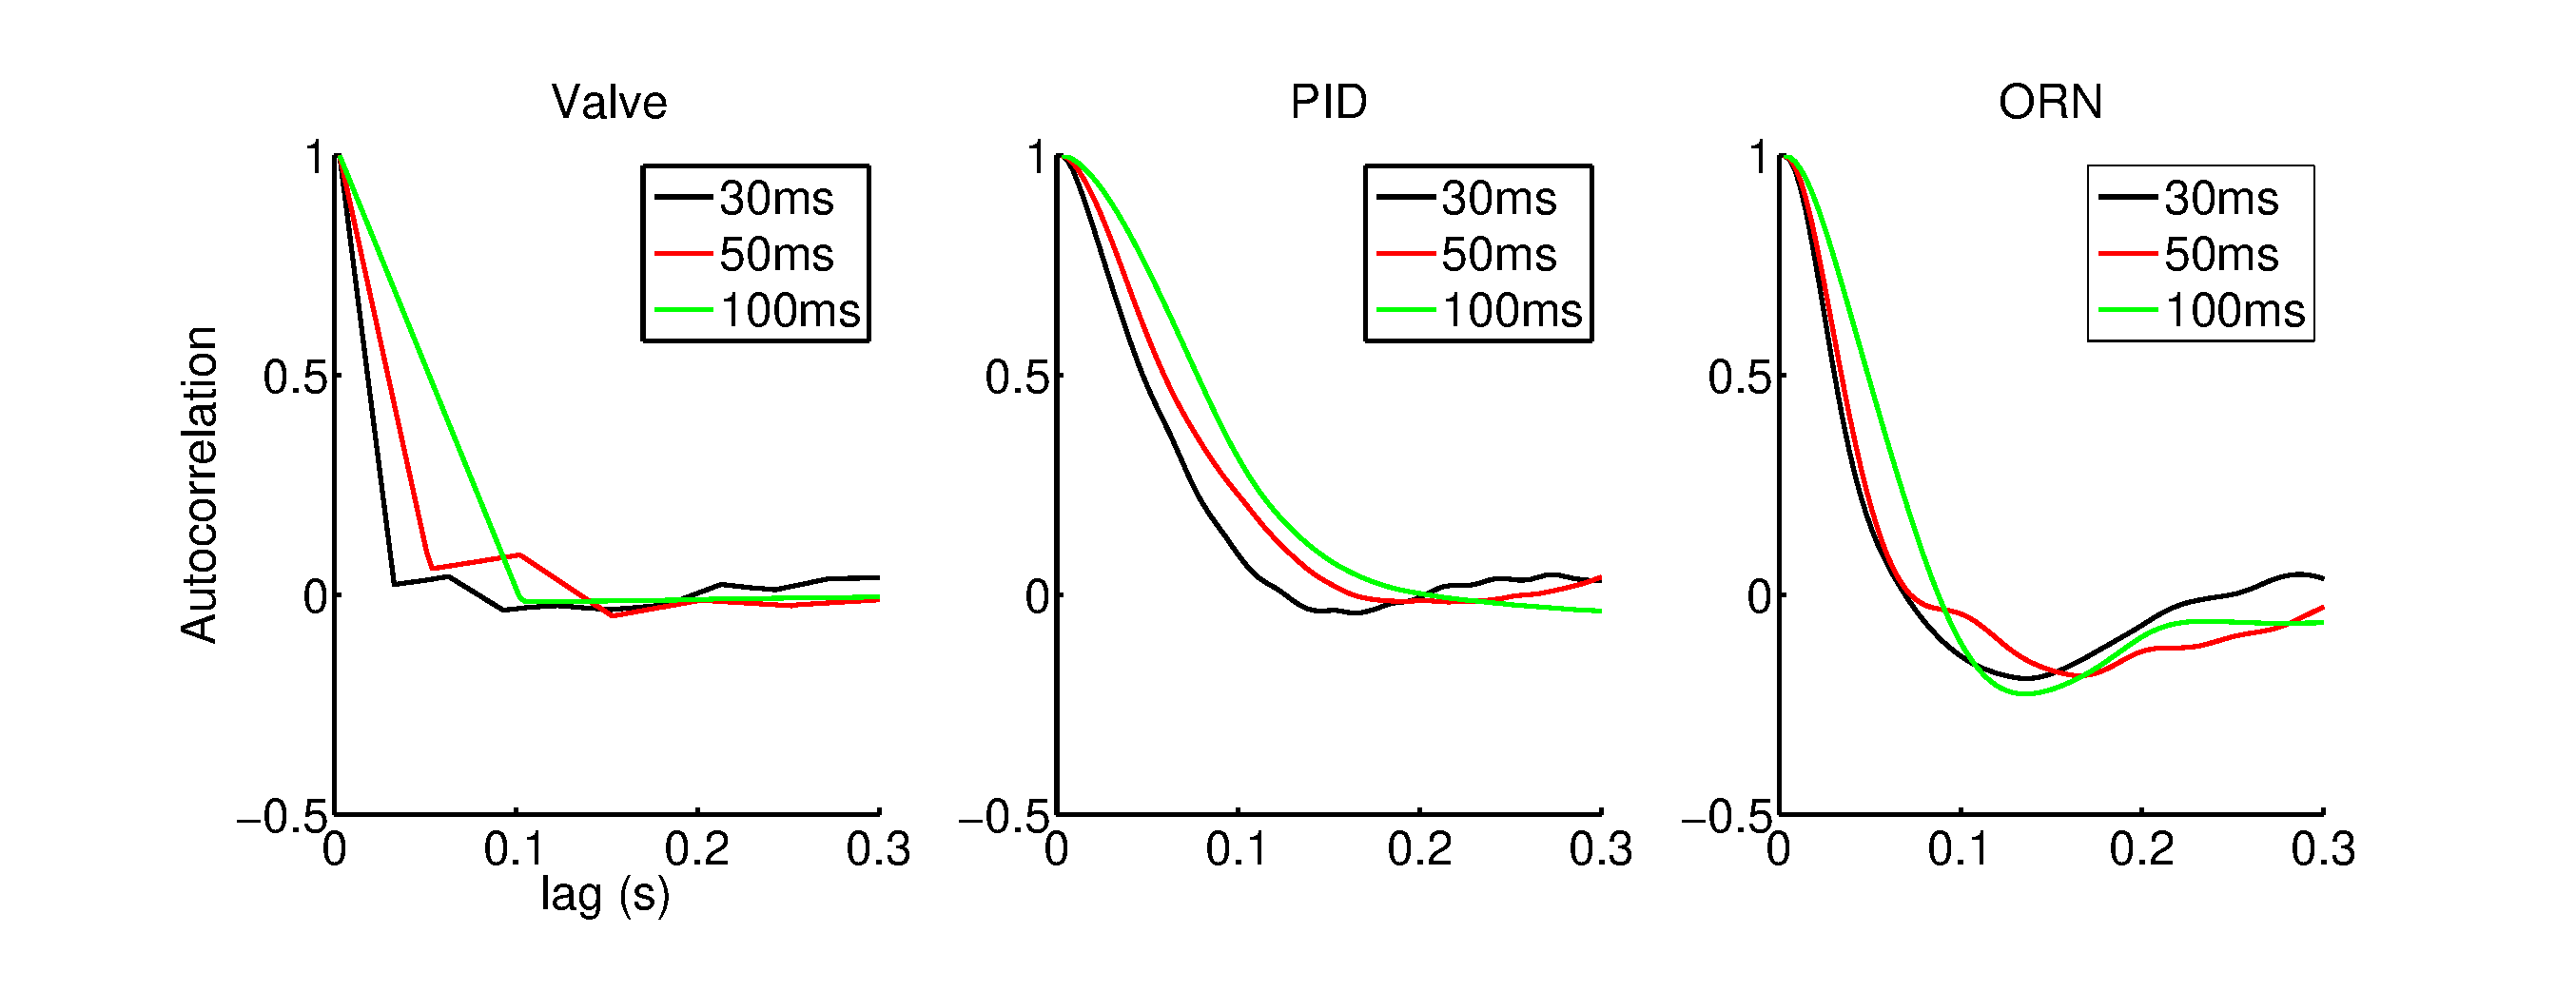
\includegraphics [width=\textwidth]{EffectOfCorrelationTime_01.pdf}


\subsection*{Are filters different for different correlations?}

\begin{par}
Now we fit filters to these data sets. In the figure below, the filters on the left are calculated using a fixed regularisation (of 1), and the filters on the right, the regularisation is varied in each case to find the "best" filter, minimising errors, high frequency components, and having a gain as close to unity as possible. In either case, we see the filters are slightly different for the three data sets; the correlation time of the stimulus seems to affect the filter we extract.
\end{par} \vspace{1em}

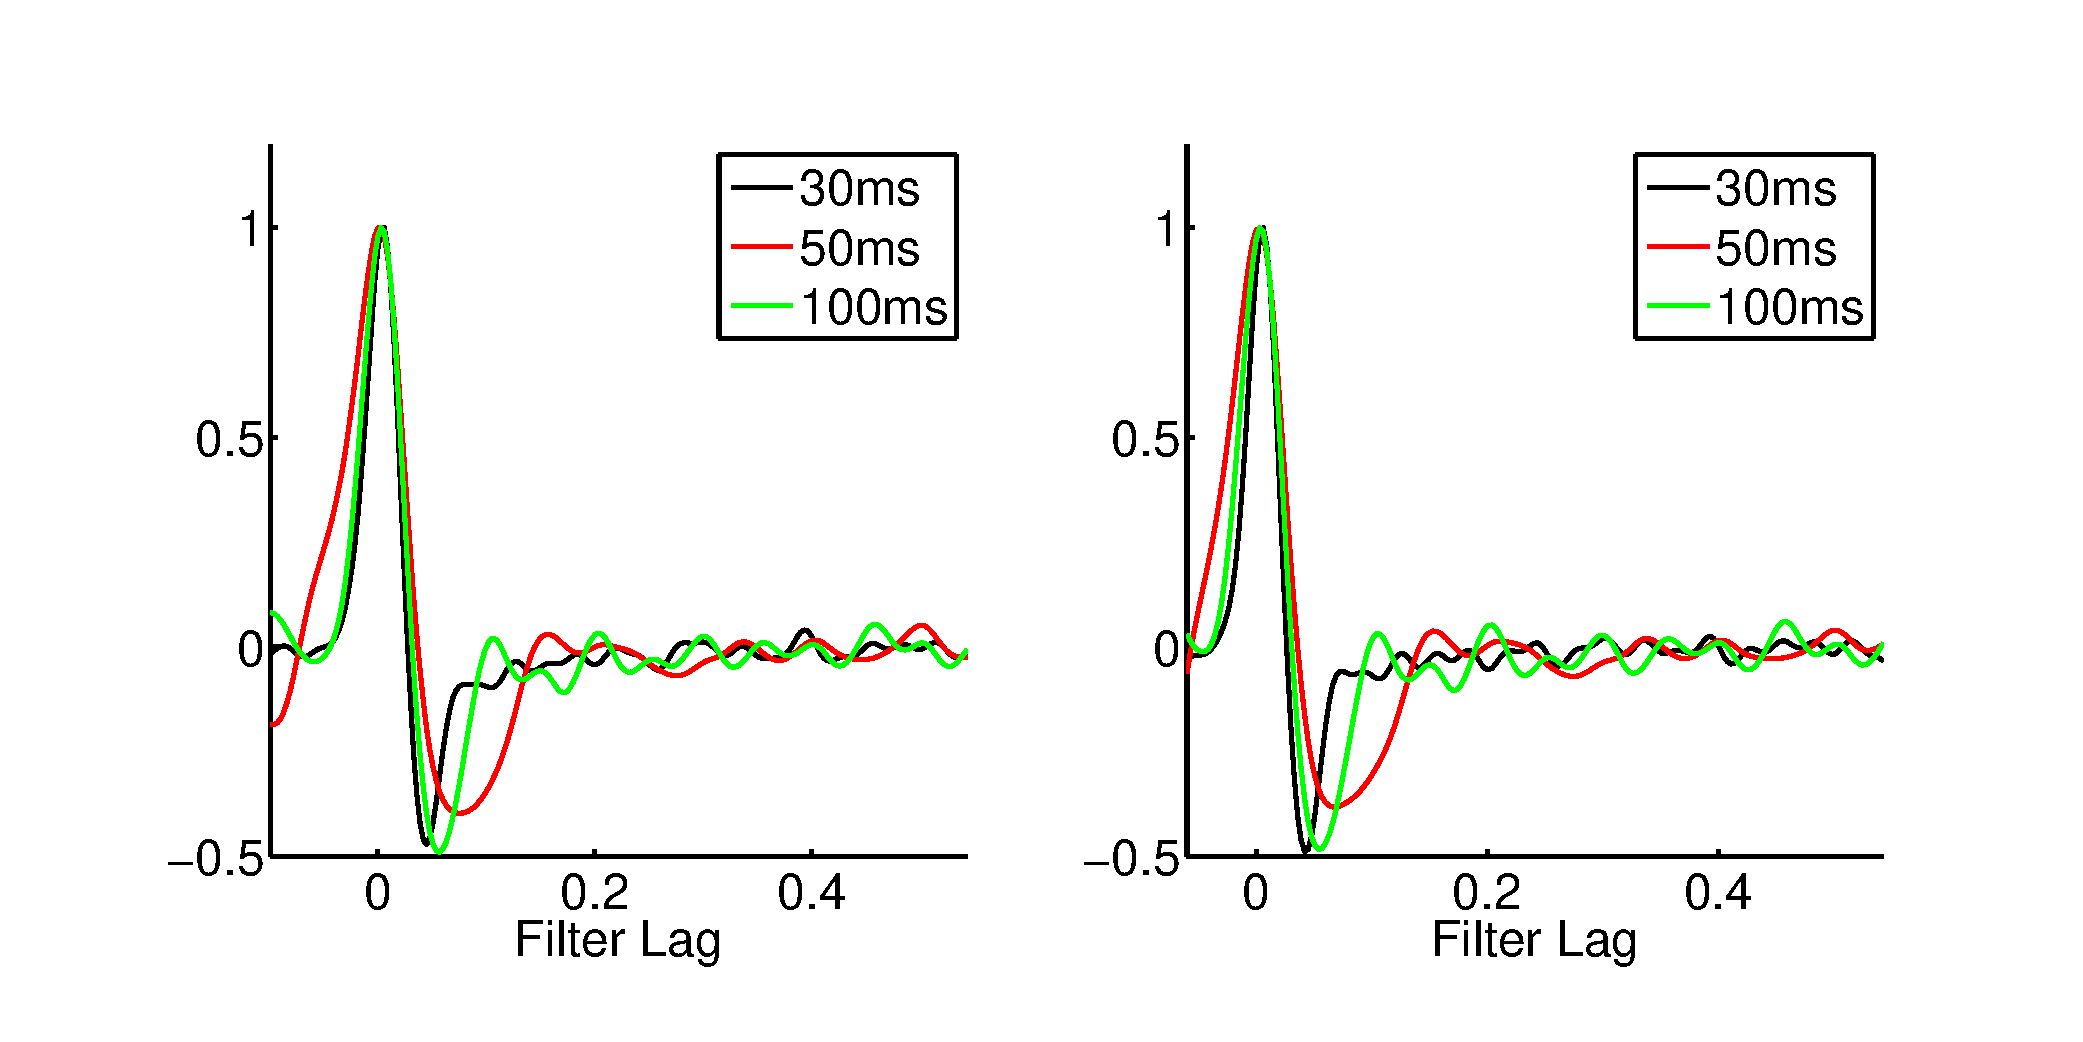
\includegraphics [width=\textwidth]{EffectOfCorrelationTime_02.pdf}
\begin{par}
These filters differ not only in their shape but also their amplitude, which is a simple scaling because the input statistics are different.
\end{par} \vspace{1em}

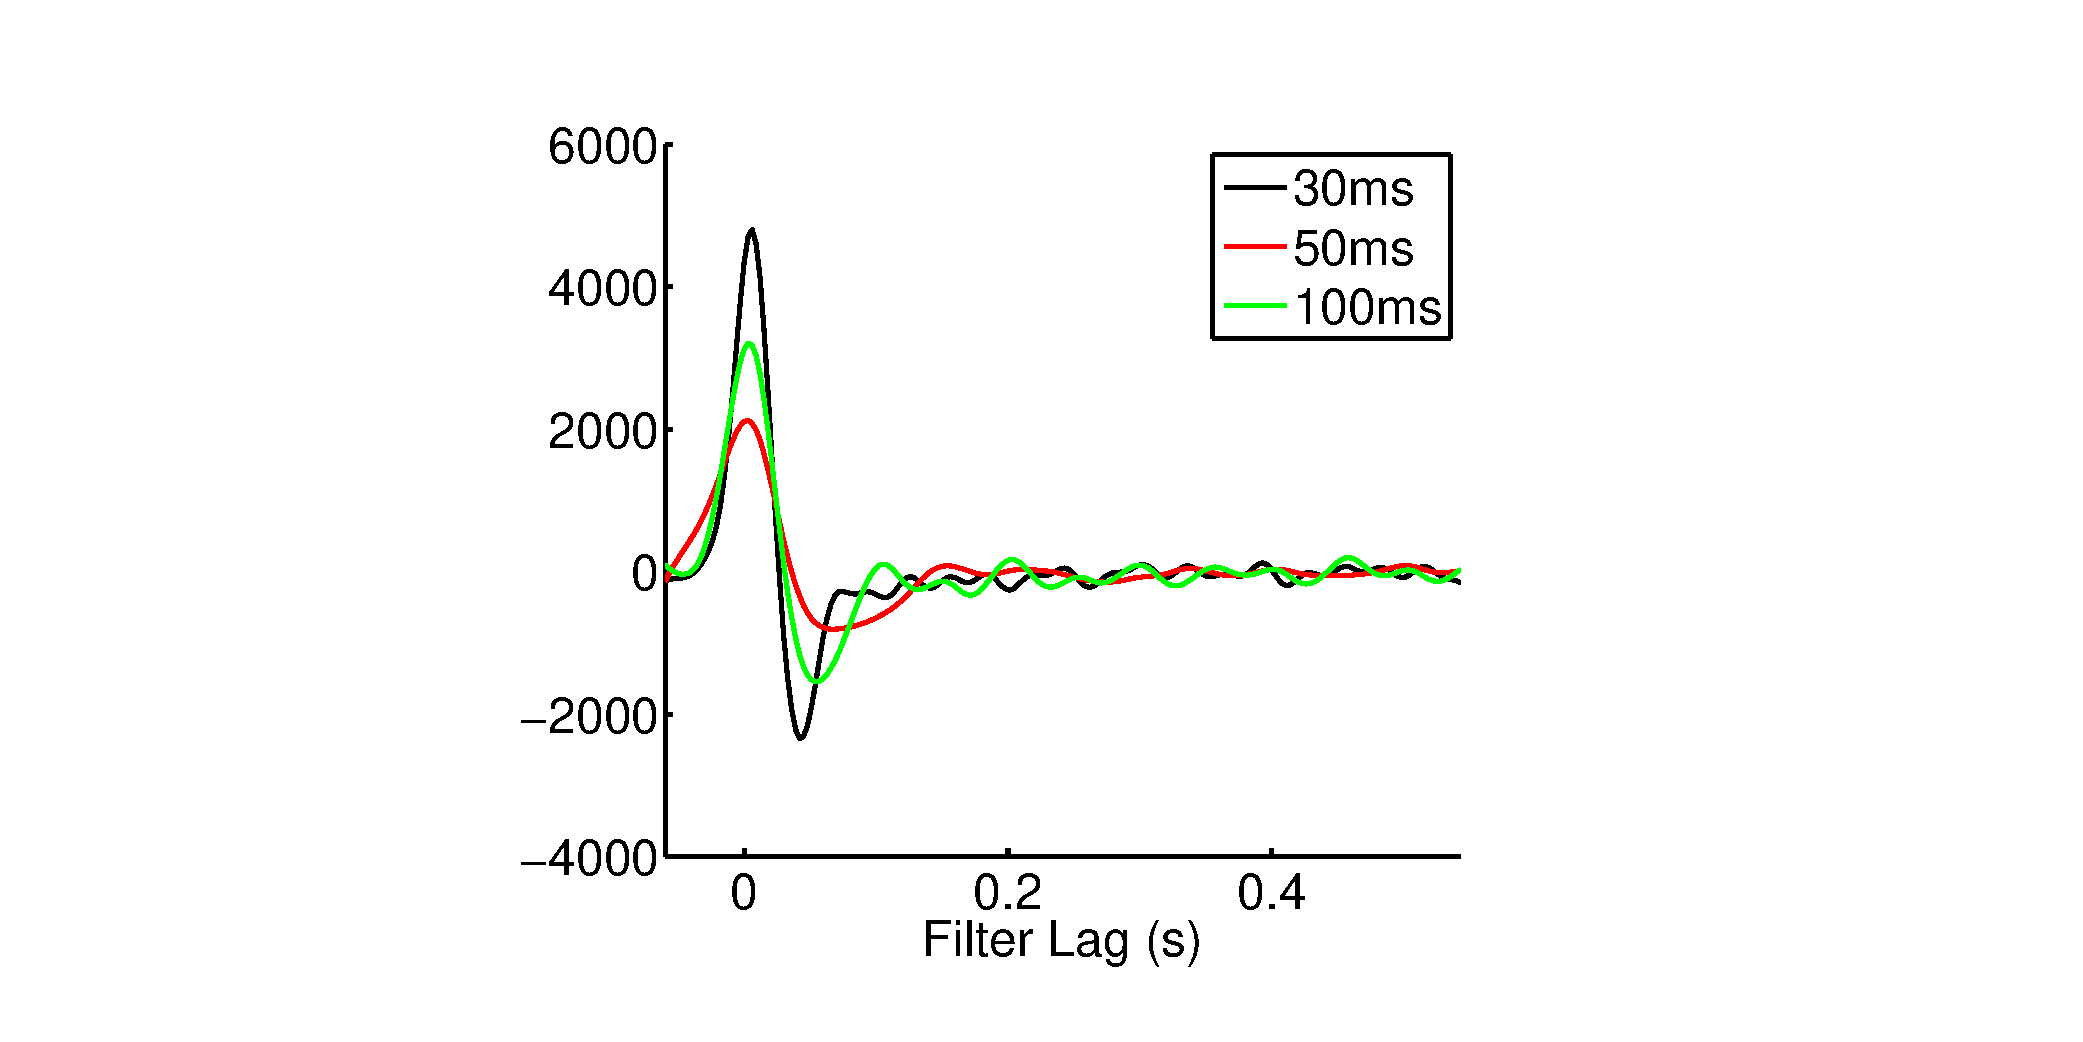
\includegraphics [width=\textwidth]{EffectOfCorrelationTime_03.pdf}
\begin{par}
Why does the filter amplitude change so much? let's look at the stimulus and the response histograms:
\end{par} \vspace{1em}

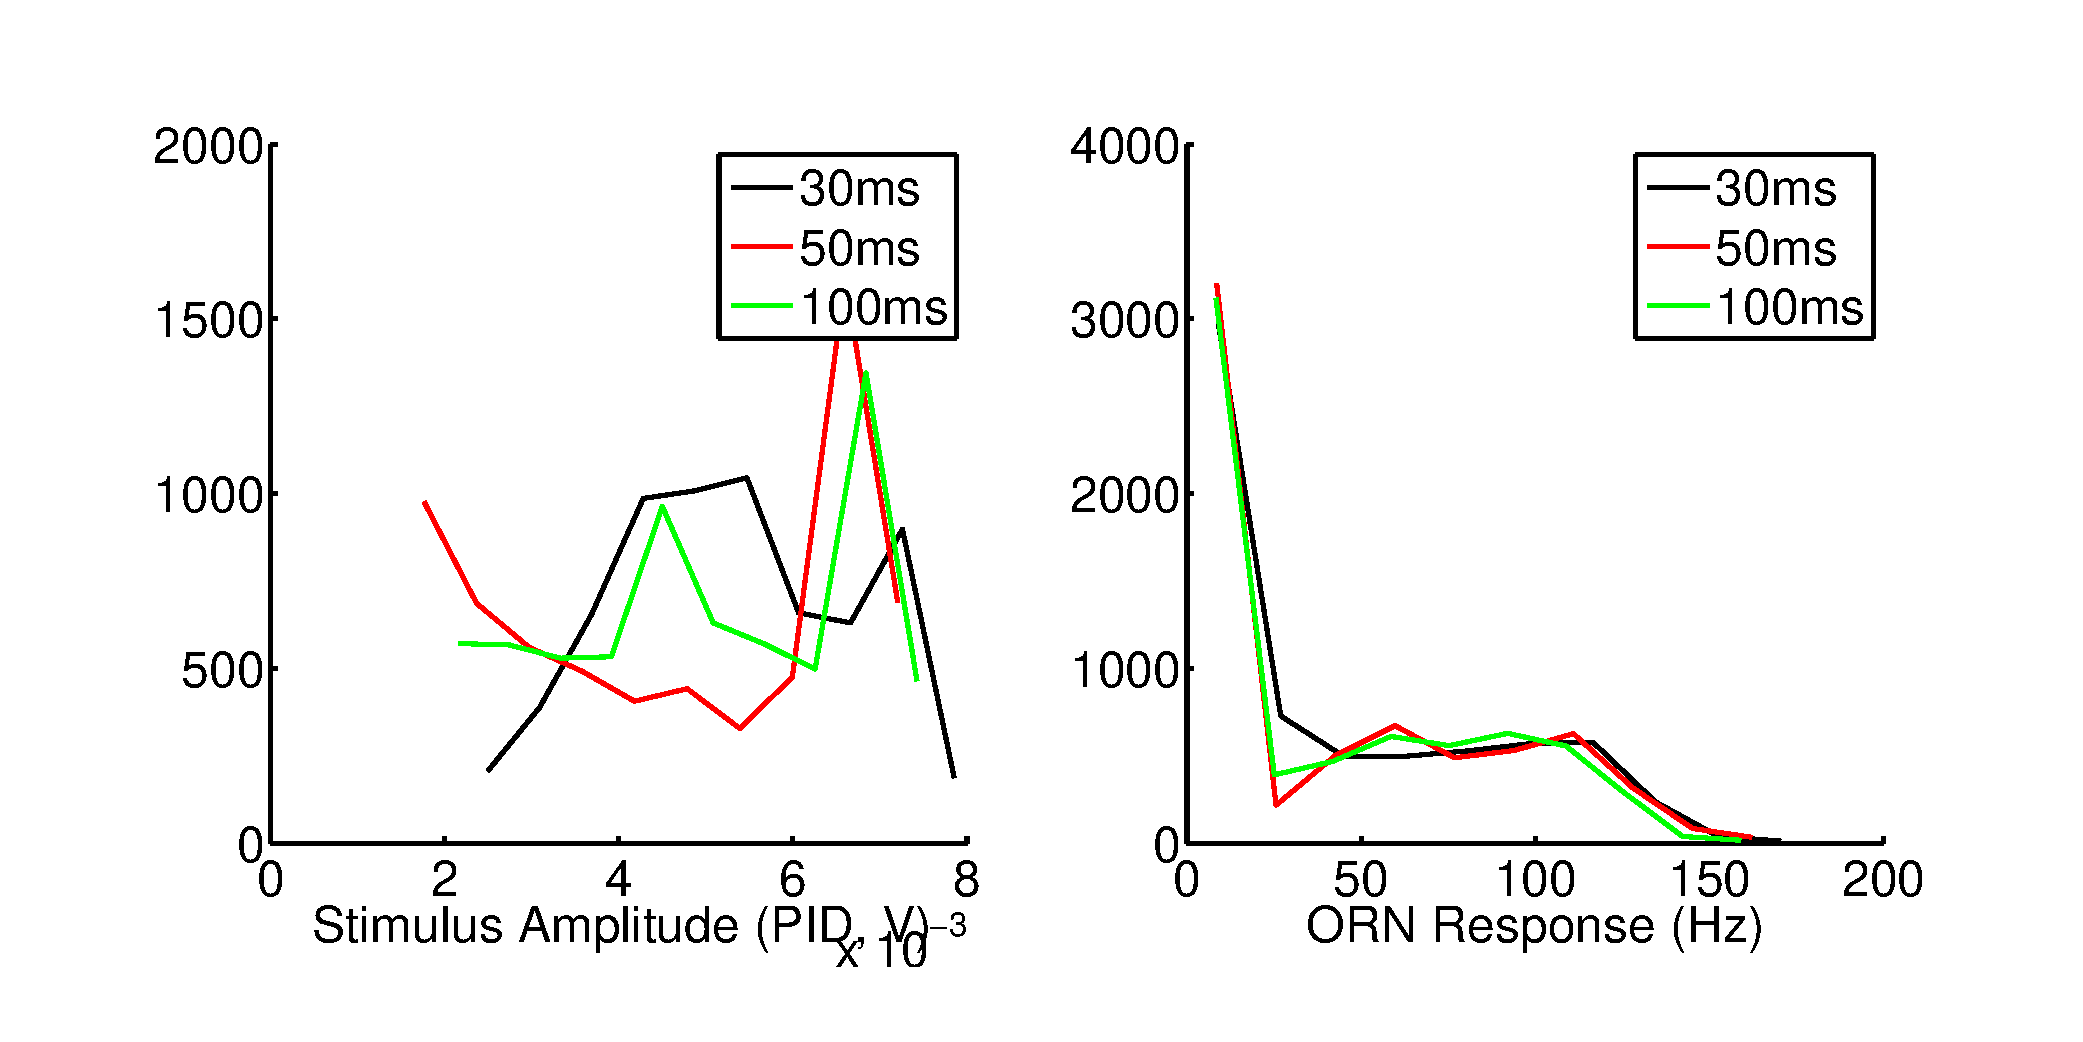
\includegraphics [width=\textwidth]{EffectOfCorrelationTime_04.pdf}


\subsection*{Cross-prediction using different filters}

\begin{par}
To disentangle the effects of filter amplitude from possible changes in filter shape, we fit a static non-linearity to the output of each linear filter and use that to predict the output.
\end{par} \vspace{1em}

        \color{lightgray} \begin{verbatim}
Local minimum possible.

lsqcurvefit stopped because the final change in the sum of squares relative to 
its initial value is less than the default value of the function tolerance.




Local minimum possible.

lsqcurvefit stopped because the final change in the sum of squares relative to 
its initial value is less than the default value of the function tolerance.




Local minimum possible.

lsqcurvefit stopped because the final change in the sum of squares relative to 
its initial value is less than the default value of the function tolerance.



\end{verbatim} \color{black}
    
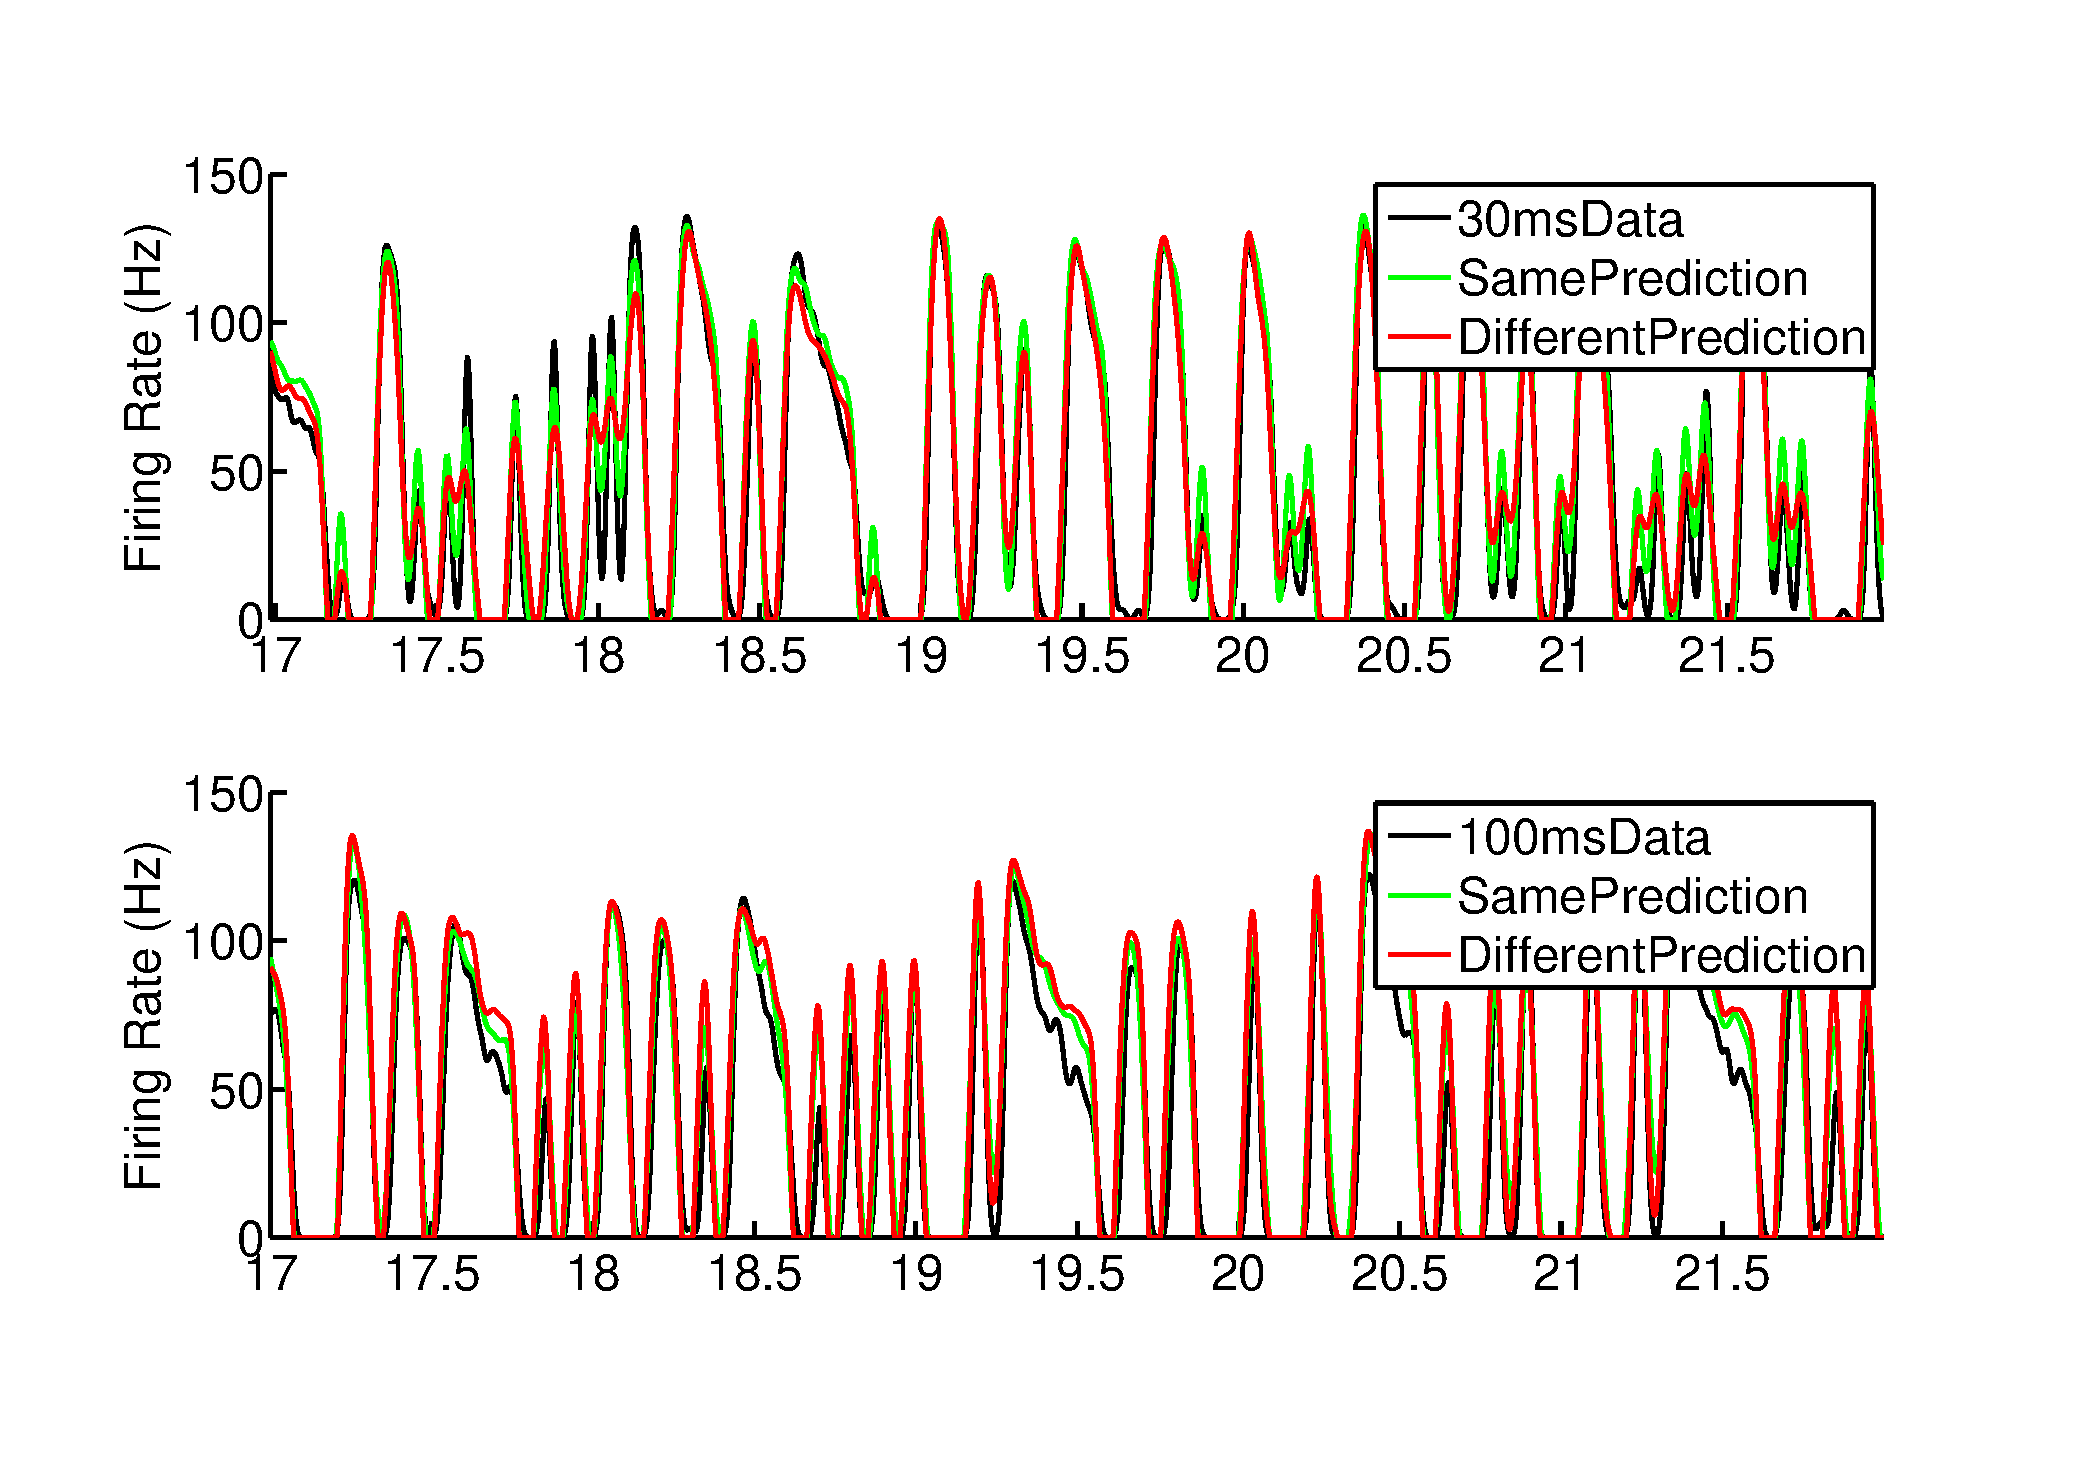
\includegraphics [width=\textwidth]{EffectOfCorrelationTime_05.pdf}
\begin{par}
How good are these filters at estimating the data? In the figure we below, we show the two extreme cases (the 30ms and 100ms correlated data) and the predictions from the filters calculated from their own data sets, along with predictions from filters calculated using the others' data. The cross-prediction filter outputs are then passed through the corresponding static non-linearities,
\end{par} \vspace{1em}

        \color{lightgray} \begin{verbatim}
Local minimum possible.

lsqcurvefit stopped because the final change in the sum of squares relative to 
its initial value is less than the default value of the function tolerance.




Local minimum possible.

lsqcurvefit stopped because the final change in the sum of squares relative to 
its initial value is less than the default value of the function tolerance.




Local minimum possible.

lsqcurvefit stopped because the final change in the sum of squares relative to 
its initial value is less than the default value of the function tolerance.




Local minimum possible.

lsqcurvefit stopped because the final change in the sum of squares relative to 
its initial value is less than the default value of the function tolerance.



\end{verbatim} \color{black}
    
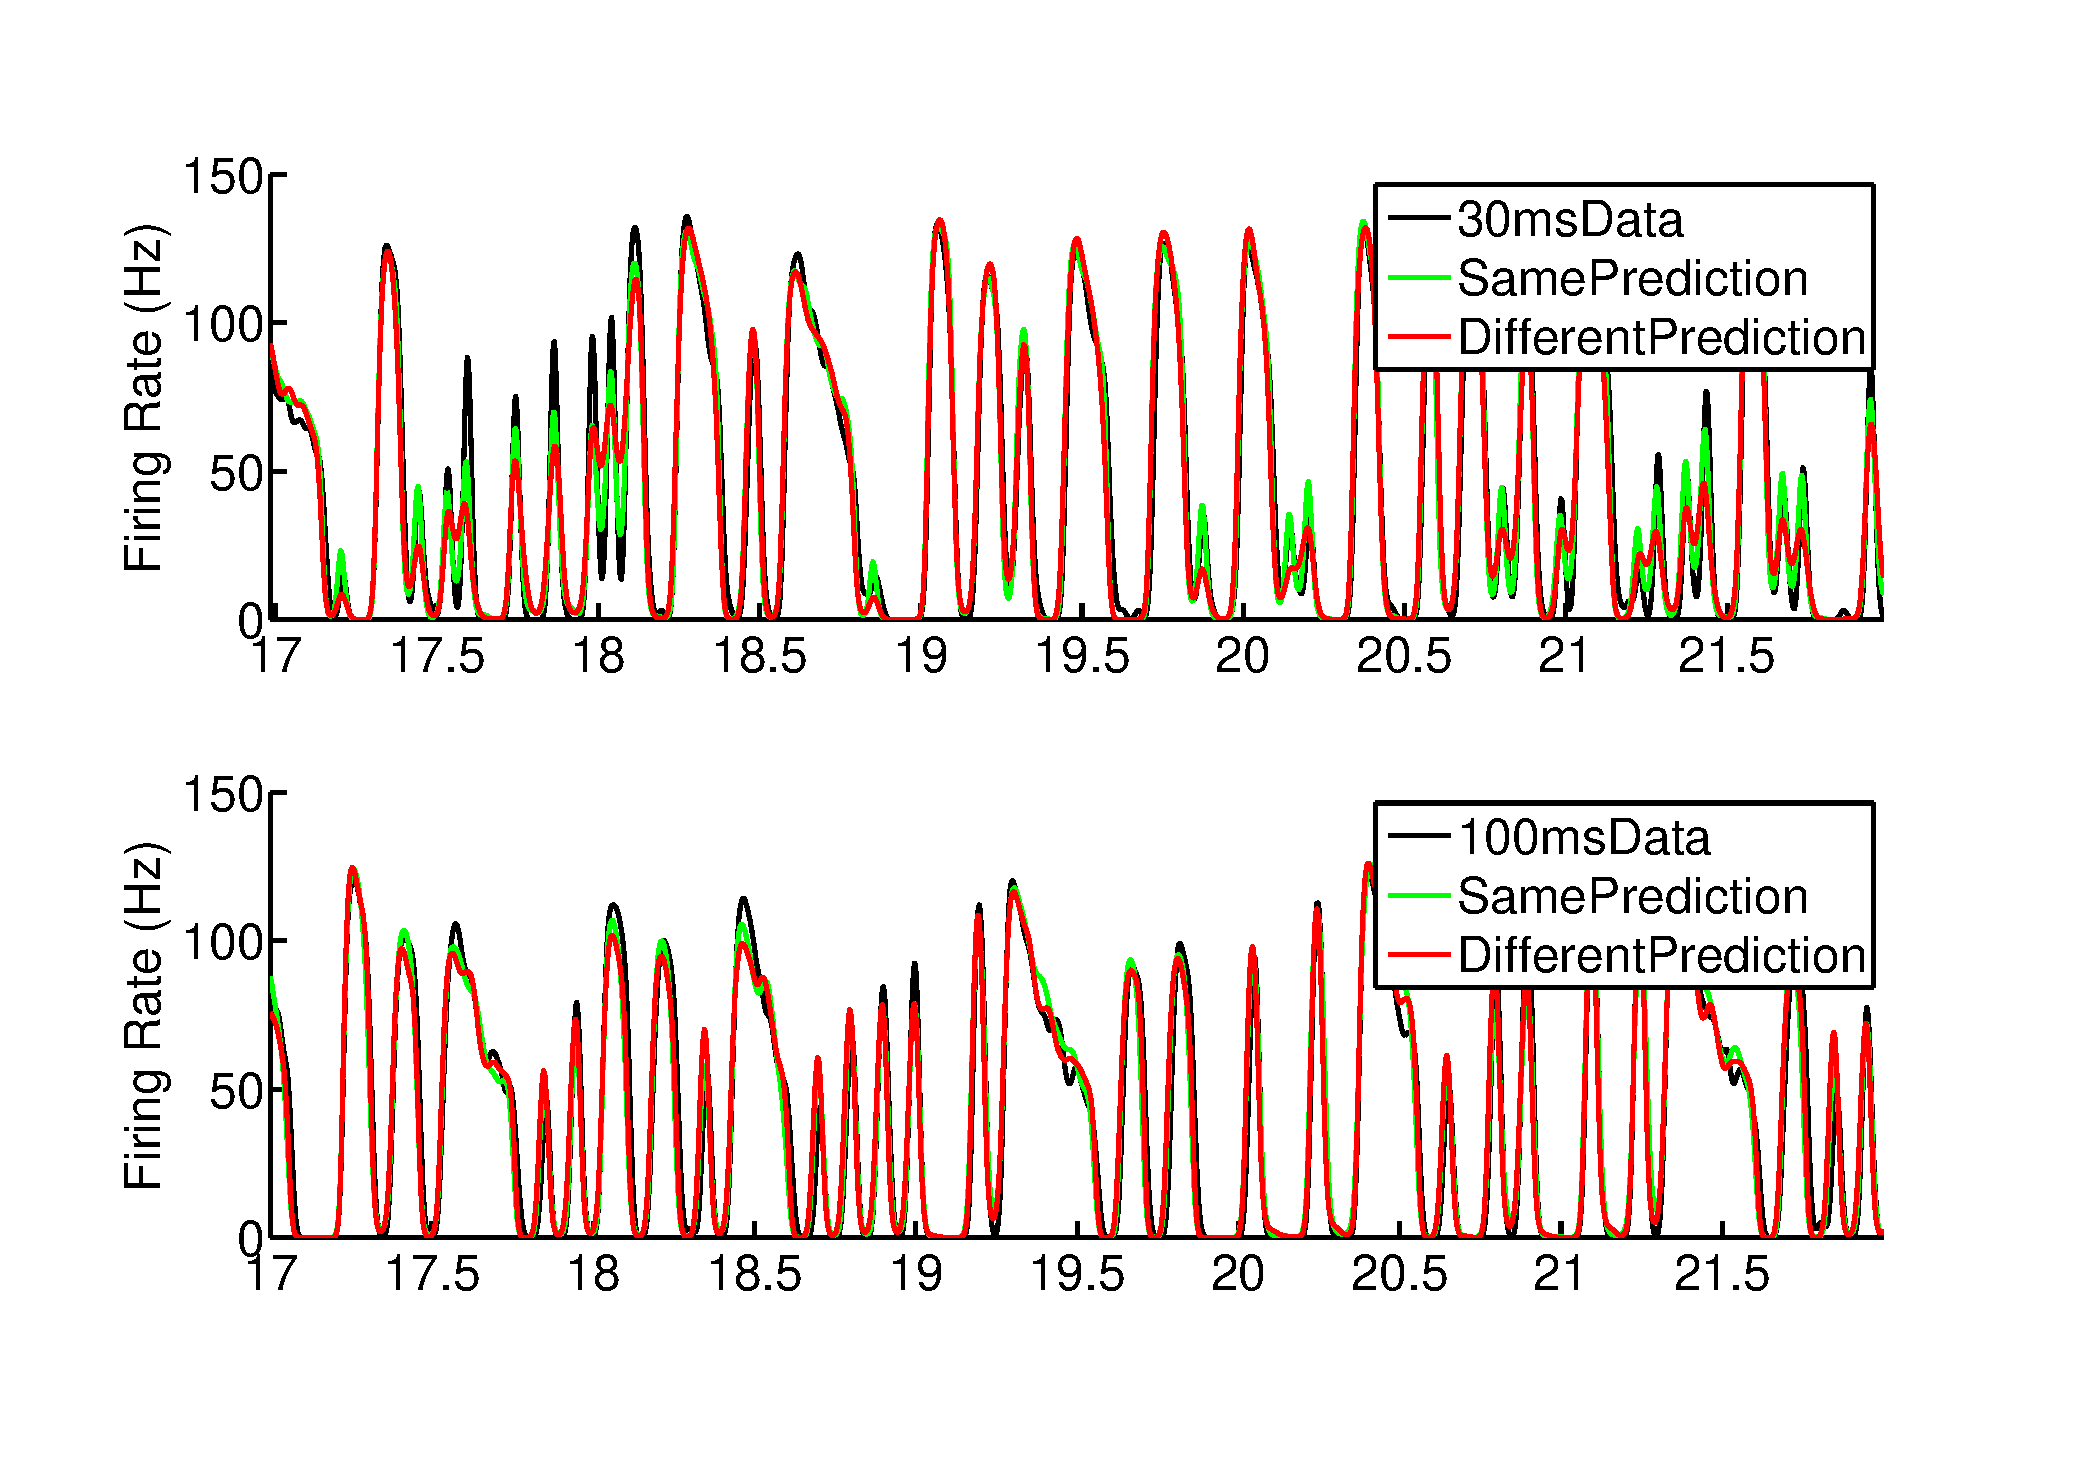
\includegraphics [width=\textwidth]{EffectOfCorrelationTime_06.pdf}
\begin{par}
How good are these cross-predictions? For the three data sets we have, we measure how well the filter from each data set predicts the data. In the matrix below, the element in ith row and jth column shows the r-square of linear prediction by the ith filter to jth data set, where the first data set has 30ms correlated stimulus, the second has 50ms correlated stimulus, and the 3rd has 100ms correlated stimulus.
\end{par} \vspace{1em}

        \color{lightgray} \begin{verbatim}    0.9344    0.9273    0.9155
    0.8365    0.9486    0.8939
    0.9137    0.9363    0.9397

\end{verbatim} \color{black}
    \begin{par}
In particular, predictions using the fastest filter outperform predictions even from filters from the same data set.
\end{par} \vspace{1em}


\subsection*{Synthetic data: filter and non-linearity estimation}

\begin{par}
What effect does using stimuli with various correlation lengths have on our estimation of the filter? Here we use a "fake" filter to represent the neuron, and pass stimuli with various correlation lengths to it, and then back out the filter from the synthetic data output.
\end{par} \vspace{1em}

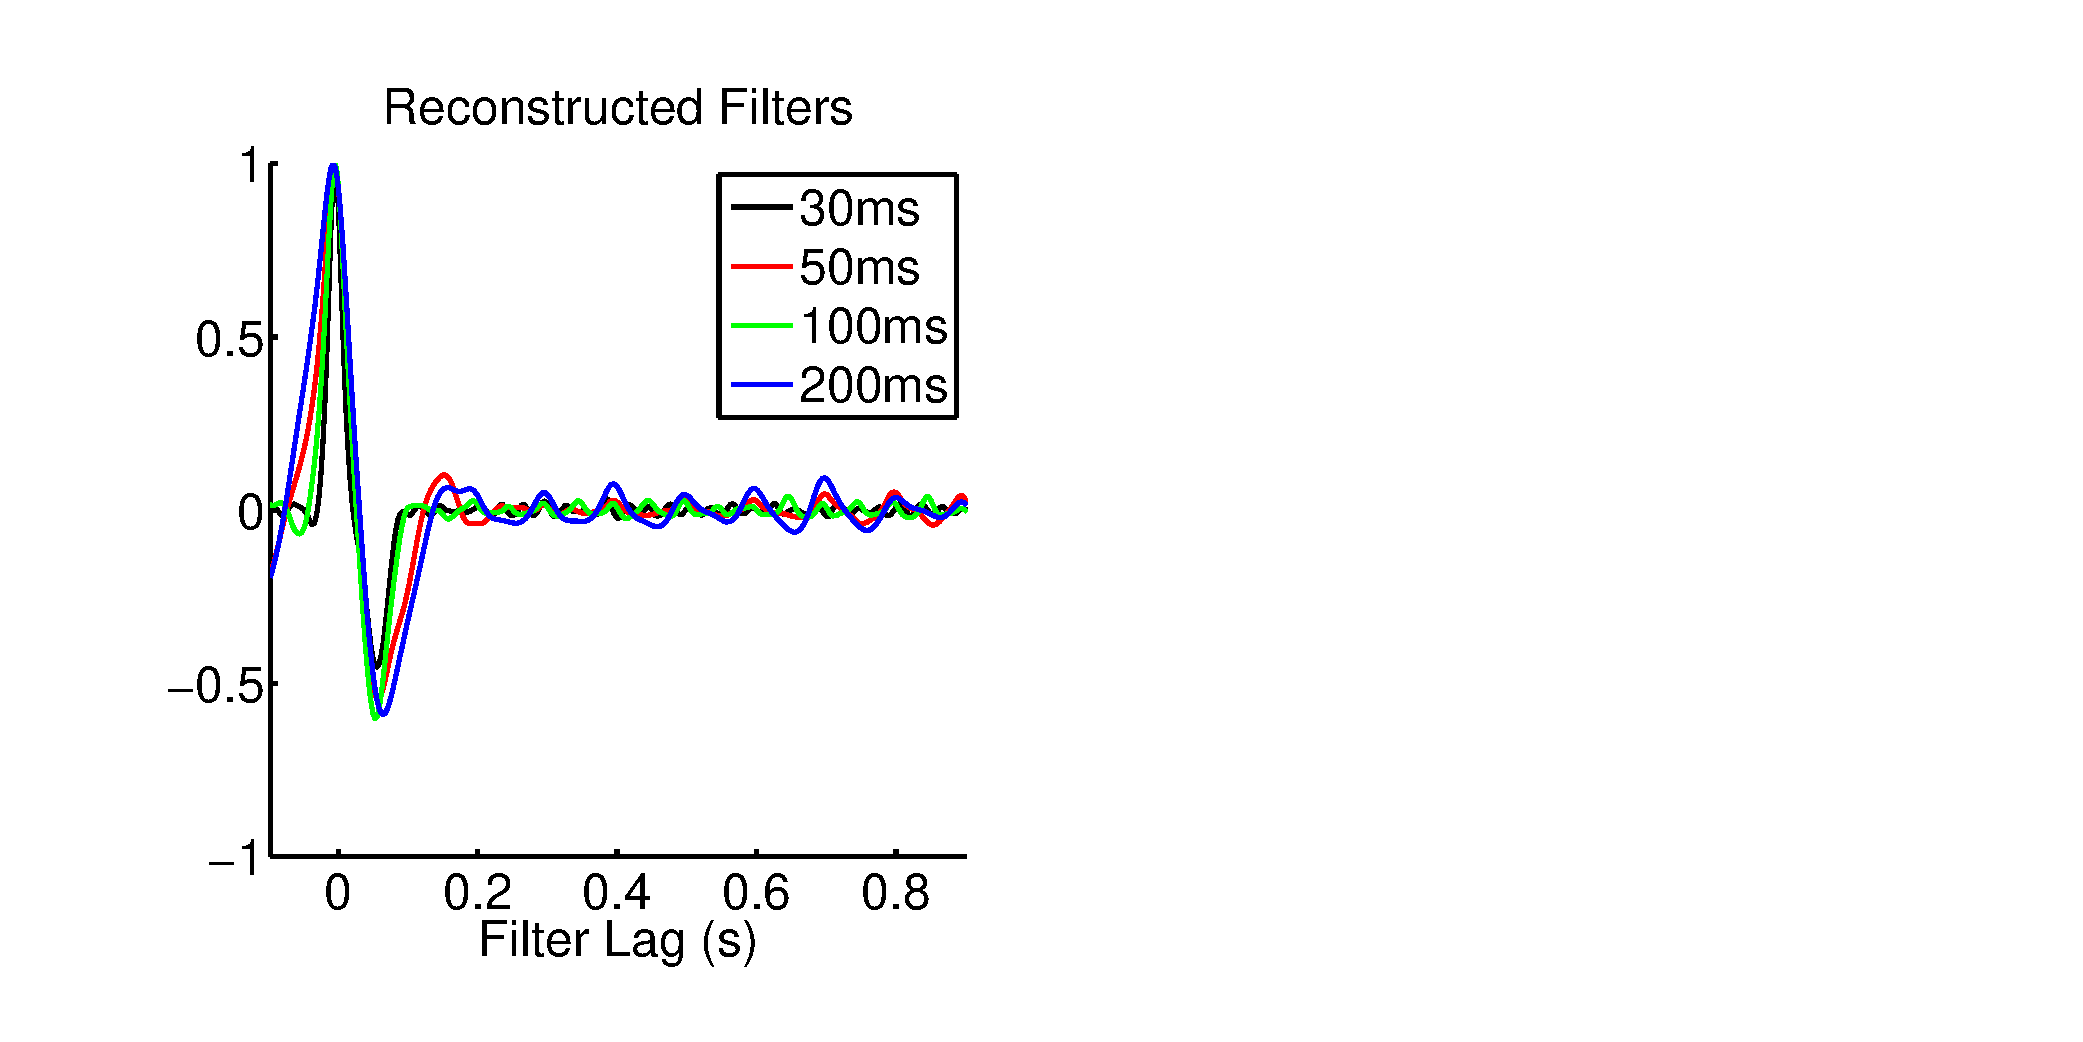
\includegraphics [width=\textwidth]{EffectOfCorrelationTime_07.pdf}



\end{document}
    
